Process aware information systems (PAIS) are becoming more and more widespread. These information systems log huge amounts of events and even more event data can be extracted from all other kinds of ubiquitous organizational databases \cite{van2015extracting}.
Additionally, in our increasingly digitized world, not just business processes are being recorded. Social media, smartphone sensors (e.g. location) and medical devices are just some of the other sources of event data nowadays.
The goal of process mining is to conduct meaningful analyses of the processes behind the event data and provide actionable results and insights.

As the basis of most process mining activities is \emph{discovering} a suitable process model. Many approaches have been developed \cite{van2016process} and current research aims to make it more scalable \cite{leemans2018scalable}.
To evaluate the quality of the discovered model with regards to the given event data, \emph{conformance checking} is used. Conformance is made up of multiple dimensions.
\begin{itemize}
    \item \emph{fitness} \textemdash \ how well is the model able to replay reality?
    \item \emph{precision} \textemdash \ does the model allow for much more behavior than reality?
    \item \emph{generalization} \textemdash \ how likely is it that new recorded data fits on the model?
    \item \emph{simplicity} \textemdash \ is the model's complexity appropriate?
\end{itemize}
Different metrics have been proposed to measure these competing dimensions \cite{van2016process} and discovery algorithms try to balance them.
For some processes a \emph{de jure} model, describing how the process should be executed may already exist.

When using a discovered or given model in conjunction with event data to diagnose the process, different perspectives can be regarded.
\begin{itemize}
    \item \emph{conformance} \textemdash \ in this context specifically, how and where does reality deviate from the model?
    \item \emph{performance} \textemdash \ are there bottlenecks in the process?
    \item \emph{data} \textemdash \ how do the attributes of event data (e.g. who executed an event) influence the process?
    \item \emph{process context} \textemdash \ how much is the process influenced by the context it is executed in? (from local like how many cases are active to external like the weather) 
\end{itemize}
State of the art approaches like \cite{mannhardt2015multi} often give overall results and averages for the entire model. For example just one fitness value. This is useful for determining if a model is has sufficient fitness but not for finding out where the deviations take place.
This is further complicated by the often dynamic nature of real-life processes. They may contain patterns of deviations and performance issues that are not constant over time. This is called concept drift. Even the interplay of all perspectives may be variable. Due to this, it is important to perform fine grained analyses of these perspectives and correlating them, e.g. by considering the \emph{time} dimension.
\begin{figure}
    \centering
    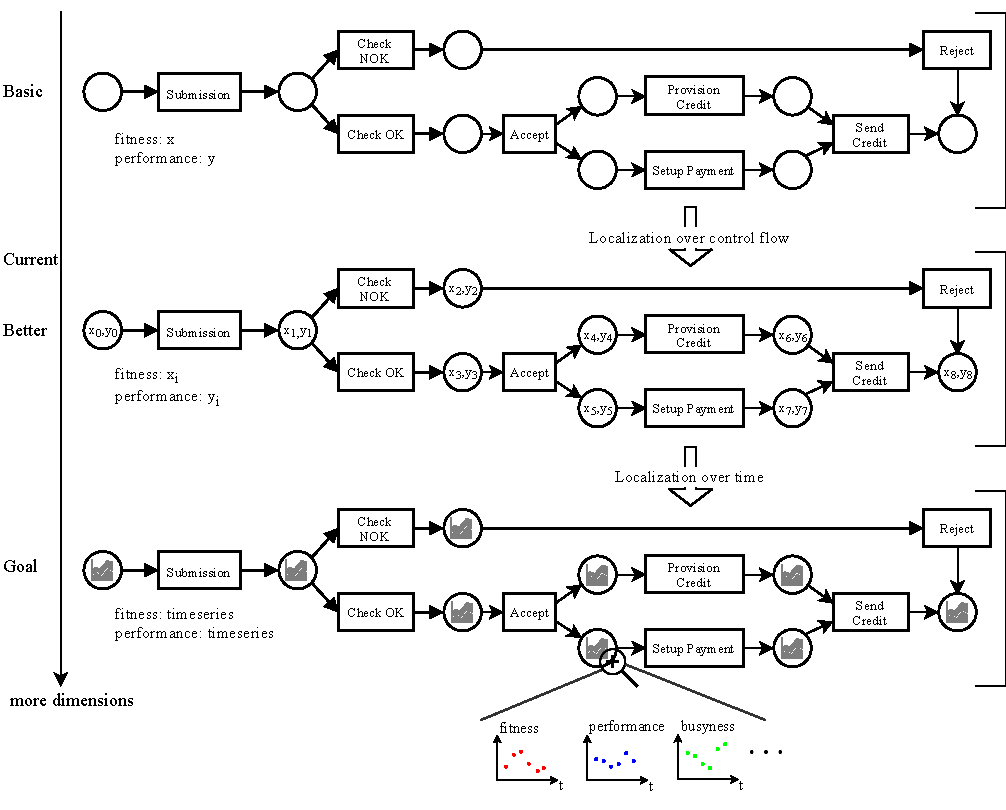
\includegraphics[width=\textwidth]{figures/introduction/bigschematic_v3.pdf}
    \caption{Schematic of the approach}
    \label{fig:bigschematic}
\end{figure}

As an example take the Petri net model given in Figure \ref{fig:bigschematic}. It describes a small credit application process where every application starts with a submission. Then, the credit history of the applicant is checked. If the result is \emph{NOK}, the application should be rejected, if not, accepted. After accepting, the credit is provisioned and the payment is setup in any order. Finally, the credit is sent. The information system logs the credit amount for cases, time and type of activity for events but no resource information. Now assume a certain employee is not following protocol. Whenever the load at his position is high and no one notices, he simply accepts low value applications where the credit history check was negative. Additionally, he actively delays high value applications, making them wait for acceptance longer. All of this only happens for a short part of the whole logged time span.

To discover such a complex pattern in full detail in the event data given the model, all perspectives are necessary. More specifically,
\begin{itemize}
    \item \emph{conformance} \textemdash \ acceptance of applications which should be rejected is a fitness problem
    \item \emph{performance} \textemdash \ the delayed applications are a performance problem
    \item \emph{data} \textemdash \ only low value applications deviate and only high value applications are delayed
    \item \emph{process context} (local) \textemdash \ all of this only happens when the affected places are busy, i.e. many cases are currently waiting there
\end{itemize}
Furthermore, these perspectives need to be measured fine grained enough. Without adding a dimension, there would only be one value per perspective for the whole log and model. For example, the average fitness, the average case duration, the case attributes and the number of cases.
By localizing the perspectives inside the model, these metrics can already differentiate at which point the problems occur. In this case after the check activities. This is an improvement but not enough to find the pattern because, due to this phenomenon only occurring for a short while, it may still be obscured by averages over the whole time span. When further localizing along the time dimension, the analysis will finally be fine enough to single out this pattern when correlating the metrics.

That is why we present an approach to approximate conformance in terms of fitness, performance and process context locally in the model and discretized over time. Figure \ref{fig:bigschematic} gives a schematic of the approach.

Chapter \ref{chap:prelim} will cover the preliminaries necessary for the approach which will be presented in Chapter \ref{chap:appr}. Following that, the implementation in ProM will be detailed in Chapter \ref{chap:impl}. Then, the approach will evaluated on a real-life event log in Chapter \ref{chap:eval}. Second to last, related work will be discussed in Chapter \ref{chap:related} and the report is concluded in Chapter \ref{chap:conclusion}.